\chapter{Network Simulator 3}
\label{chap:ns3}

The \textit{ns-3} simulator is an open, extensible discrete-event network simulator designed primarily 
for educational and network research purposes \cite{ns3}.

In summary, \textit{ns-3} provides models of how packet data networks work and operate, as well as a 
simulation engine that allows users to run simulation experiments. To do research that are 
more difficult or impossible to do with real systems, to examine system behavior in a highly 
controlled, reproducible setting, and to understand about how networks work.

\textit{ns-3} is a collection of modules that can be used together as well as with other software 
libraries. This tool works mainly at the command line on \textit{Linux} or \textit{MacOS} and with 
\textit{C++} and \textit{Python} programming languages and development tools.

\section{Getting Started}
\label{sec:ns3intro}

The prerequisites for the \textit{ns-3} release version 3.32 are the following tools:

\begin{table}[h]
  \centering
  \begin{tabular}{@{}ll@{}}
  \toprule
  Prerequisite & Package/version                             \\ \midrule 
  C++ compiler & \texttt{clang++} or \texttt{g++} (\texttt{g++} version 4.9 or greater) \\[-0.8em]
  Python       & \texttt{python3}  version \textgreater{}= 3.5         \\ [-0.8em]
  Git          & any recent version                          \\ [-0.8em]
  tar          & any recent version                          \\ [-0.8em]
  bunzip2      & any recent version                          \\ \bottomrule \\[-0.8em]
  \end{tabular}
  \caption{Prerequisites for ns-3}
\end{table}

Start by downloading the source archive from \href{https://www.nsnam.org/release/ns-allinone-3.32.tar.bz2}{nsnam}
or \href{https://gitlab.com/nsnam/ns-3-allinone.git}{gitlab}. Then build \textit{ns-3} with \texttt{build.py}:

\begin{lstlisting}[language=myshell,caption={Download and installation of ns-3}, captionpos=b]
  # Download from nsnam
  $ cd
  $ mkdir workspace
  $ cd workspace
  $ wget https://www.nsnam.org/release/ns-allinone-3.32.tar.bz2
  $ |\color{myblue}tar| xjf ns-allinone-3.32.tar.bz2
  $ cd ns-allinone-3.32
  # Building ns-3
  $ ./build.py --enable-examples --enable-tests
  # Running a script
  # Create or copy a script to the scratch directory
  $ cp examples/tutorial/first.cc scratch/myfirst.cc
  $ ./waf --run scratch/myfirst
\end{lstlisting}

\section{ns-3 Concepts}
\label{sec:ns3conc}
This section will go over several networking concepts that have a specific meaning in ns-3.

\begin{itemize}[topsep=0pt]
  \item[] \textbf{Node}: A \texttt{Node} in \textit{ns-3} is the basic computing device abstraction. 
  The \texttt{Node} class has methods for managing computing device representations in simulations.
  \item[] \textbf{Application}: A \textit{ns-3} application run on \textit{ns-3} \texttt{Nodes}. An 
  \texttt{Applicacion} is the basic abstraction for a user program that generates some simulated activity.  
  The \texttt{Application} class provides functions for controlling the representations of the simulated
  version of user-level applications.
  \item[] \textbf{Channel}: A \texttt{Channel} in \textit{ns-3} is an abstraction of the basic communication 
  subnetwork in which \texttt{Nodes} are connected in. It can be as simple as a wire or as complicated as a
  large Ethernet switch.
  \item[] \textbf{Net Device}: A \texttt{NetDevice} in \textit{ns-3} simulates a \textit{Network Interface Card (NIC)}
  and the software controlling the \textit{NIC}. A \texttt{NetDevice} is installed in a \texttt{Node} to allow 
  it to communicate over \texttt{Channels} with other \texttt{Nodes} in the simulation.
  \item[] \textbf{Helpers}: Helper objects are created to make some commun tasks easier. Such as connecting
  \texttt{NetDevices} to \texttt{Nodes}, \texttt{NetDevices} to \texttt{Channels}, assigning IP addresses, etc. 
\end{itemize}

\section{Logging Module}
Message logging is a basic feature for large softwares, and \textit{ns-3} is no different. \textit{ns-3} 
offer a complete module for message logging with configurable verbosity levels. This means that logging 
functions of specific components can be enabled and other can be disabled completely.

There are different levels of log messages of ascending verbosity defined in \textit{ns-3}:

\begin{itemize}[topsep=0pt]
  \item \textbf{\texttt{LOG\_ERROR}}: For error messages (associated function: \texttt{NS\_LOG\_ERROR}).
  \item \textbf{\texttt{LOG\_WARN}}: For warning messages (associated function: \texttt{NS\_LOG\_WARN}).
  \item \textbf{\texttt{LOG\_DEBUG}}: For relatively rare, ad-hoc debugging messages (associated function: \texttt{NS\_LOG\_DEBUG}).
  \item \textbf{\texttt{LOG\_INFO}}: For informational messages about program progress (associated function: \texttt{NS\_LOG\_INFO}).
  \item \textbf{\texttt{LOG\_FUNCTION}}: For messages describing each function called (two associated function: \texttt{NS\_LOG\_FUNCTION}
  used for member functions, and \texttt{NS\_LOG\_FUNCTION\_NOARGS}, used for static functions)).
  \item \textbf{\texttt{LOG\_LOGIC}}: For messages describing logical flow within a function (associated function: \texttt{NS\_LOG\_LOGIC}).
  \item \textbf{\texttt{LOG\_ALL}}: Log everything mentioned above (no associated function).
\end{itemize}

To enable all logs, it is as simple as modifying a shell variable. In the next example the logging for the class
\texttt{UdpEchoClientApplication} and \texttt{UdpEchoServerApplication} is enabled with all levels, the time 
and the function prefixes:

\begin{lstlisting}[escapechar=@, language=myshell,caption={Enabling logging in ns-3}, captionpos=b]
  $ export 'NS_LOG=UdpEchoClientApplication=level_all|prefix_func|prefix_time:UdpEchoServerApplication=level_all|prefix_func|prefix_time'
\end{lstlisting}

To disable logging simply type:

\begin{lstlisting}[escapechar=@, language=myshell,caption={Disabling logging in ns-3}, captionpos=b]
  $ export NS_LOG=
\end{lstlisting}

For more information with the logging modure see \cite{ns3}.

\section{Command Line Arguments}
There are local and global variables that can be changed in the command line without
editing the scripts. An example of a command could be like this:

\begin{lstlisting}[escapechar=@, language=myshell,caption={Command line arguments}, captionpos=b]
  # To check help 
  $ ./waf --run "scratch/myfirst --PrintHelp"
  # To check variables for PointToPointNetDevice
  $ ./waf --run "scratch/myfirst --PrintAttributes=ns3::PointToPointNetDevice"
  # We set the Datarate to 5Mbps
  $ ./waf --run "scratch/myfirst --ns3::PointToPointNetDevice::DataRate=5Mbps"
\end{lstlisting}

\section{Tracing System}
The main goal of the simulations is to extract and generate output, and \textit{ns-3} offers two
mechanisms for this. Also, since \textit{ns-3} is a C++ software, using \texttt{std::cout} for
output is also available.

\subsection{ASCII Tracing}
ns-3 includes helper function that encapsulates the low-level tracing system and guides you 
through the technicalities of establishing some simple packet traces. If you enable this feature, 
the output will be in ASCII files, hence the name.

To enable ASCII Tracing, right before the call to \texttt{Simulator::Run ()}, add the following lines
of code:

\begin{lstlisting}[escapechar=@, language=myC++,caption={ASCII tracing}, captionpos=b]
  AsciiTraceHelper ascii;
  pointToPoint.EnableAsciiAll (ascii.CreateFileStream ("out.tr"));
\end{lstlisting}

This will generate the output from \texttt{pointToPoint} to a file named \texttt{out.tr}.

\subsection{PCAP Tracing}
The ns-3 device helpers can also create \texttt{.pcap} trace files. The \textit{pcap} file
contains the packets captured during the simulation. \textit{Wireshark} or \textit{tcpdump} 
are programs capable of reading and visualizing \textit{pcap} files.

To enable \textit{pcap} tracing simply add:
\begin{lstlisting}[escapechar=@, language=myC++,caption={PCAP tracing}, captionpos=b]
  pointToPoint.EnablePcapAll ("myfirst");
\end{lstlisting}

This will create various \texttt{.pcap} files in the format \texttt{"myfirst-0-0.pcap"}, meaning
the trace file for node 0 and device 0.

\section{ns-3 Modules \& Models}
In this section, modules used in this thesis will be presented, based on the official
manual from \cite{ns3}. But first, It is 
essential to understand the difference between modules and models:

% \begin{itemize}[noitemsep,topsep=0pt]
\begin{itemize}[itemsep=0pt, topsep=0pt]
  \item \textbf{Modules} are the different libraries that form \textit{ns-3}.
  \item \textbf{Models} are the simulated, abstract representations of real-life objects,
  protocols, devices, etc.
\end{itemize}

As the reader may already know, \textit{ns-3} is modular. A new module will be introduced in 
the \autoref{chap:abrmodule} as a result of this Master final project.

\subsection{Antenna Module}
The Antenna module provides a \texttt{AntennaModel} base class as an interface for radiation
pattern modelling of an antenna. Also, there are a set of classes derived from this base
class that implements types of antennas with differente radiation patterns.

\subsubsection{AntennaModel}
The \texttt{AntennaModel} uses a coordinate system as shown in the \autoref{fig:ns3antenna}. This
model uses, for a point ${p}$ in the space with Cartesian coordinates used by the \texttt{MobilityModel},
the coordinates ${(x,y,z)}$ and transforms into spherical coordinates ${(r,\theta,\phi)}$.

The radiation pattern is express as a mathematical function ${g(\theta,\phi) \rightarrow \R}$

\begin{figure}[h]
  \centering
  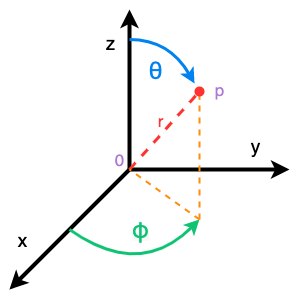
\includegraphics[width=0.35\textwidth]{img/antennamodel.png}
  \caption{Coordinate system of the AntennaModel. Source: nsnam \cite{ns3}}
  \label{fig:ns3antenna}
\end{figure}

\begin{itemize}[itemsep=0pt, topsep=0pt]
  \item \textbf{IsotropicAntennaModel} 
  
  The \texttt{IsotropicAntennaModel} is onmidirectional, this means that the radiation pattern have
  a 0dB gain for all direction.
  \item \textbf{CosineAntennaModel}
  
  The antenna gain of the \texttt{CosineAntennaModel} is defined as:
  \begin{equation}
    g(\phi,\theta)=cos^n \bigg( \frac{\phi-\phi_0}{2} \bigg)
  \end{equation}

  with ${\phi_0}$ as the antenna's azimuthal orientation, this is, the direction of maximum gain. And the exponential
  \begin{equation}
    n=-\frac{3}{20\,log_{10} \big( cos\frac{\phi_{3dB}}{4} \big) }
  \end{equation}

  determines the wanted 3db beamwidth ${\phi_{3dB}}$.
  \item \textbf{ParabolicAntennaModel}

  In the \texttt{ParabolicAntennaModel}, the antenna gain is determined as:
  \begin{equation}
    g(\phi,\theta)=-min \bigg( 12 \bigg( \frac{\phi-\phi_0}{\phi_{3dB}}^2 \bigg) ,A_{max} \bigg)
  \end{equation}
  where ${A_{max}}$ is the maximum attenuation in dB of the antenna. 
\end{itemize}

\subsection{Buildings Module}
The Buildings module provide various models, but these are more relevant for this thesis:

\subsubsection{Building class}

The \texttt{Building} model implements and tries to simulate real-life buildings, which affects
wireless communications in different ways.

A \texttt{Building} can be residential, office or commertial, has different types of external
wall (wood, concrete with/out windows, stone blocks), has a number of floors and rooms in each floor.

Some limitations have to be made:
\begin{itemize}[topsep=0pt]
  \item A \texttt{Building} is represented as a rectangular parallelepiped.
  \item The walls needs to be parallel to the cardinal coordinates.
  \item A \texttt{Building} is a grid of rooms, with z axis as the floor number and the x and y room
  indexes start from 1 and increses along the x and y axis.
  \item All the rooms are the same size.
\end{itemize}

\subsubsection{MobilityBuildingInfo class}

The \texttt{MobilityBuildingInfo} keeps track of the mobility and positional information of 
the nodes with respect to buildings in a simulation. A node can be inside or outside of
a building and if the node is indoors, this class knows in which building and in which room
the node is positioned.

\subsubsection{ItuR1238PropagationLossModel}

This class provides an ITU P.1238-based building-dependent indoor propagation loss model 
that includes losses owing to building type (i.e., residential, office and commercial). 
The following is the analytical expression:

\begin{equation}
  L_{total} = 20\,log\,f + N\,log\,d + L_f (n) - 28[dB]
\end{equation}

where ${N}$ is the power loss coefficient, ${L_f}$ is the loss depending of type of building,
${f}$ is the frequency [MHz] and ${d}$ is de distance [m].

\subsubsection{BuildingPropagationLossModel}

The \texttt{BuildingsPropagationLossModel} adds a set of pathloss model elements that are 
building-dependent and can be used to design various pathloss logics. The elements of the 
pathloss model are discussed in the subsections below.

\begin{itemize}
  \item \textbf{External Wall Loss}

  This component simulates the loss of communication from indoors to outdoors and vice versa through walls.
  \item \textbf{Internal Wall Loss}

  This component simulates the loss of penetration in indoor-to-indoor communications within a single building.
  \item \textbf{Height Gain Model}

  This component simulates the gain caused by the transmitting equipment being on a higher floor than the ground.
  \item \textbf{Shadowing Model}

  The shadowing is represented using a log-normal distribution with a variable standard deviation
  as a function of the MobilityModel instances' relative position (inside or outdoor). For each 
  pair of MobilityModels, a single random value is generated and remains constant during the 
  simulation. As a result, the model is only suitable for static nodes.
\end{itemize}

\subsubsection{Pathloss logics}
The pathloss logic provided by inheriting from \texttt{BuildingsPropagationLossModel}
is described in the following sections.
\begin{itemize}
  \item \textbf{HybridBuildingPropagationLossModel}

  In order to imitate multiple outdoor and interior circumstances, as well as indoor-to-outdoor 
  and outdoor-to-indoor scenarios, the \texttt{HybridBuildingsPropagationLossModel} was created by 
  combining various well-known pathloss models. In particular, this class combines the pathloss 
  models listed below:

  \item \textbf{OhBuildingPropagationLossModel}
  This is a simpler propagation loss model. It uses the \texttt{OkumuraHataPropagationLossModel} and 
  also taking account the pathloss elements of the \texttt{BuildingPropagationLossModel}.
\end{itemize}

\subsection{Internet Module}
This module includes the implementations of TCP/IP related components like IPv4, ARP, UDP, TCP and so on.
A \texttt{Node} with the Internet Stack installed is called a Internet Node.

In order to use the Internet Protocol, a node should be assigned an IP address. It can be done manually
or through the \textit{Dynamic Host Configuration Protocol (DHCP)}.

Full bidirectional TCP with connection setup and close logic is supported by the native ns-3 TCP model.
Various TCP congestion algorithms are also available, such as New Reno, Cubic, HighSpeed, etc.


\subsection{Mobility Module}


\subsection{Network Module}
? sockets???


\subsection{PointToPoint NetDevice}


\subsection{LTE Module}
There are two main components in the LTE-EPC simulation model.

\begin{itemize}[topsep=0pt, noitemsep]
  \item \textbf{LTE Model}. Include models for the UE and the eNodeB nodes. Also the LTE Radio Protocol
  Stack (PHY, MAC, RLC, etc.).

  \item \textbf{EPC Model}. Include models for the entities, interfaces and protocols in the Evolver Packet Core.
\end{itemize}

\subsubsection{LteHelper}
The \texttt{LteHelper} is a helper which manages the LTE radio access network's 
configuration as well as the setup and release of EPS bearers. The API definition and 
implementation are both provided by the \texttt{LteHelper} class.

This is a code snipper to create UEs and eNodeBs with \texttt{LteHelper}:

\begin{lstlisting}[language=myC++,caption={LteHelper usage}, captionpos=b]
  // Create LteHelper and the nodes
  Ptr<LteHelper> lteHelper = CreateObject<LteHelper> ();
  NodeContainer enbNodes;
  enbNodes.Create (1);
  NodeContainer ueNodes;
  ueNodes.Create (2);

  // Set the mobility model
  MobilityHelper mobility;
  mobility.SetMobilityModel ("ns3::ConstantPositionMobilityModel");
  mobility.Install (enbNodes);
  mobility.SetMobilityModel ("ns3::ConstantPositionMobilityModel");
  mobility.Install (ueNodes);

  // Install NetDevices to the nodes
  NetDeviceContainer enbDevs;
  enbDevs = lteHelper->InstallEnbDevice (enbNodes);
  NetDeviceContainer ueDevs;
  ueDevs = lteHelper->InstallUeDevice (ueNodes);  

  // Attach UEs to the eNodeB
  lteHelper->Attach (ueDevs, enbDevs.Get (0));
\end{lstlisting}

\begin{itemize}
  \item \textbf{Network Attachment}
  
  To connect an UE to the network, the UE needs to be attached to an eNodeB. This is done by calling the
  \texttt{LteHelper::Attach} function. The are two possible ways for network attachment.

  \begin{itemize}
    \item[$\circ$] \textbf{Automatic Attachment}

    This method uses the \textit{Strengh of the Received Signal (RSRP)} as the criteria to choose 
    , in the initial cell selection process, which eNodeB to connect to. The automatic attachment 
    works by calling:

    \begin{lstlisting}[language=myC++,caption={UE Automatic Attachment}, captionpos=b]
    lteHelper->Attach (ueDevs); // attach one or more UEs to a strongest cell
    \end{lstlisting}
    
    \item[$\circ$] \textbf{Manual Attachment}
    Alternatively, selecting the eNodeB at the beginning of the simulation is also possible:

    \begin{lstlisting}[language=myC++,caption={UE Manual Attachment}, captionpos=b]
    lteHelper->Attach (ueDevs, enbDev); // attach one or more UEs to a single eNodeB
    \end{lstlisting}
  \end{itemize}

  \item \textbf{Simulation Output}
  
  The LTE module offer PHY, MAC, RLC, and PDCP level \textit{Key Performance Indicators (KPI)}
  that can be enabled using \textbf{LteHelper}:

  \begin{lstlisting}[language=myC++,caption={Enable LTE trace outputs}, captionpos=b]
    lteHelper->EnablePhyTraces ();
    lteHelper->EnableMacTraces ();
    lteHelper->EnableRlcTraces ();
    lteHelper->EnablePdcpTraces ();
  \end{lstlisting}
\end{itemize}

\subsubsection{EpcHelper}
The \texttt{EpcHelper} allows the simulation of the Evolve Packet Core. The usage of EPC with 
LTE devices allows for IPv4 and IPv6 networking. To put it another way,it is possible to use 
standard ns-3 apps and sockets across IPv4 and IPv6 via LTE, as well as connect an LTE network 
to any other IPv4 and IPv6 network in the simulation.

\begin{lstlisting}[language=myC++,caption={Enable Evolved Packet Core}, captionpos=b]
  Ptr<LteHelper> lteHelper = CreateObject<LteHelper> ();
  Ptr<PointToPointEpcHelper> epcHelper = CreateObject<PointToPointEpcHelper> ();
  lteHelper->SetEpcHelper (epcHelper);
\end{lstlisting}


Emulation mode

\subsubsection{MAC}
// MAC scheduler 
// AMC 
// CQI

\subsection{UE PHY Measurements Model}

\subsubsection{Mobility Model with Buildings}
// manual y tutorial

\subsubsection{AntennaModel \& MIMO Model}

\subsubsection{Radio Environment Maps}



\subsection{Configuration parameters}
// por completar
\begin{lstlisting}[language=myshell, caption={Configuration parameters}, captionpos=b]
  default ns3::LteHelper::Scheduler "ns3::PfFfMacScheduler"
  default ns3::LteHelper::PathlossModel "ns3::FriisSpectrumPropagationLossModel"
  default ns3::LteEnbNetDevice::UlBandwidth "25"
  default ns3::LteEnbNetDevice::DlBandwidth "25"
  default ns3::LteEnbNetDevice::DlEarfcn "100"
  default ns3::LteEnbNetDevice::UlEarfcn "18100"
  default ns3::LteUePhy::TxPower "10"
  default ns3::LteUePhy::NoiseFigure "9"
  default ns3::LteEnbPhy::TxPower "30"
  default ns3::LteEnbPhy::NoiseFigure "5"
\end{lstlisting}

REM

LTE enb phy

UM buffer size

TCP new reno?

Lossmodel

Fading loss model

Earfcn

Building